% !TeX TXS-program:compile = txs:///arara
% arara: lualatex: {shell: no, synctex: yes, interaction: batchmode}
% arara: pythontex: {rerun: modified} if found('pytxcode', 'PYTHONTEX#py')
% arara: lualatex: {shell: no, synctex: yes, interaction: batchmode} if found('pytxcode', 'PYTHONTEX#py')
% arara: lualatex: {shell: no, synctex: yes, interaction: batchmode} if found('log', '(undefined references|Please rerun|Rerun to get)')

\documentclass[a4paper,11pt]{article}
\usepackage[revgoku]{cp-base}
\graphicspath{{./graphics/}}
%variables.
\donnees[classe={1\up{ère} 2M2},matiere={[SPÉ.MATHS]},mois={Jeudi 05 Mai},annee=2022,typedoc=TEST~,numdoc=8,duree={20 minutes}]
%formatage
\author{Pierquet}
\title{\nomfichier}
\hypersetup{pdfauthor={Pierquet},pdftitle={\nomfichier},allbordercolors=white,pdfborder=0 0 0,pdfstartview=FitH}
%divers
\lhead{\entete{Durée : \duree}}
\chead{\entete{\lycee}}
\rhead{\entete{\classe{} - \mois{} \annee}}
\lfoot{\pied{\matiere}}
\cfoot{\logolycee{}}
\fancypagestyle{sujetA}{\fancyhead[R]{\entete{\classe{}A - \mois{} \annee}}}
\fancypagestyle{sujetB}{\fancyhead[R]{\entete{\classe{}B - \mois{} \annee}}}

\begin{document}

\pagestyle{fancy}

\part{TEST08 - Produit scalaire}%SUJETA

\setcounter{numexos}{0}

\medskip

\nomprenomtcbox

\medskip

\exonum{}

\begin{enumerate}
	\item Déterminer $\vect{AB}\cdot\vect{AC}$ avec comme données $AB=7$ ; $AC=4$ et $\widehat{BAC}=30^{\circ}$.
	
	{\hfill\papierseyes*{20}{2}\hfill~}
	\item On considère la figure suivante, dans laquelle trois carrés de côté 2 sont mis côte à côte.
	
	\begin{center}
		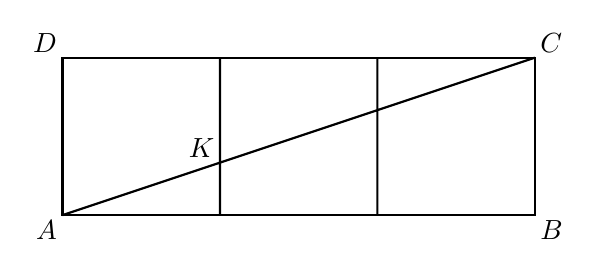
\begin{tikzpicture}[inner sep=2pt,outer sep=0pt]
			\draw[thick] (0,0) rectangle (6,2) ;
			\draw[thick] (2,0)--(2,2) (4,0)--(4,2) (0,0)--(6,2) ;
			\draw (0,0) node[below left] {$A$} ;
			\draw (6,0) node[below right] {$B$} ;
			\draw (6,2) node[above right] {$C$} ;
			\draw (0,2) node[above left] {$D$} ;
			\draw (2,0.667) node[above left] {$K$} ;
		\end{tikzpicture}
	\end{center}

	Déterminer, en justifiant, la valeur de $\vect{AB}\cdot\vect{AD}$ et la valeur de $\vect{AB}\cdot\vect{AK}$.
	
	{\hfill\papierseyes*{10}{2}~~\papierseyes*{10}{2}\hfill~}
	\item Déterminer $\vect{u}\cdot\vect{v}$ puis $\vect{u}^2$ avec comme données $\vect{u}\coordeux{3}{5}$ et $\vect{v}\coordeux{-7}{4}$.
	
	{\hfill\papierseyes*{10}{2}~~\papierseyes*{10}{2}\hfill~}
	\item Soit $x$ un réel et soient $\vect{u}\coordeux{x}{4}$ et $\vect{v}\coordeux{3}{-2}$ deux vecteurs.
	\begin{enumerate}
		\item Déterminer la valeur de $x$ de sorte que $\vect{u}$ et $\vect{v}$ soient orthogonaux.
		\item Déterminer la valeur de $x$ de sorte que $\vect{u}$ et $\vect{v}$ soient colinéaires.
	\end{enumerate}
	
	{\hfill\papierseyes*{10}{3}~~\papierseyes*{10}{3}\hfill~}
\end{enumerate}

\medskip

\exonum{}

\medskip

Dans un repère orthonormé, on considère les trois poins $A(1\,;\,-2)$ ; $B(5\,;\,-3)$ et $C(3\,;\,6)$.

\begin{enumerate}
	\item Déterminer les coordonnées des vecteurs $\vect{AB}$, $\vect{AC}$ et $\vect{BC}$.
	\item Calculer $\vect{AB}\cdot\vect{AC}$ puis en déduire la nature du triangle $ABC$.
\end{enumerate}

{\hfill\papierseyes*{10}{3}~~\papierseyes*{10}{3}\hfill~}

\end{document}